% Part 7: Parallelization with Agents
% A Comprehensive Guide to Agentic Coding Tools
% University of South Carolina - Beamer Presentation

\documentclass[aspectratio=169,11pt]{beamer}

% ============================================================================
% PACKAGES
% ============================================================================
\usepackage[utf8]{inputenc}
\usepackage[T1]{fontenc}
\usepackage{lmodern}
\usepackage{amsmath,amssymb,amsfonts}
\usepackage{graphicx}
\usepackage{tikz}
\usetikzlibrary{shapes.geometric, arrows.meta, positioning, calc, fit, backgrounds, matrix, decorations.pathreplacing}
\usepackage{listings}
\usepackage{booktabs}
\usepackage{array}
\usepackage{multirow}
\usepackage{xcolor}
\usepackage{fontawesome5}
\usepackage{hyperref}

% ============================================================================
% UofSC COLOR DEFINITIONS
% ============================================================================
% Primary Colors
\definecolor{UofSCGarnet}{HTML}{73000a}
\definecolor{UofSCBlack}{HTML}{000000}
\definecolor{UofSCWhite}{HTML}{ffffff}

% Accent Colors
\definecolor{UofSCRose}{HTML}{CC2E40}
\definecolor{UofSCAtlantic}{HTML}{466A9F}
\definecolor{UofSCCongaree}{HTML}{1F414D}
\definecolor{UofSCHorseshoe}{HTML}{65780B}
\definecolor{UofSCGrass}{HTML}{CED318}
\definecolor{UofSCHoneycomb}{HTML}{A49137}

% Neutral Colors
\definecolor{UofSC90Black}{HTML}{363636}
\definecolor{UofSC70Black}{HTML}{5C5C5C}
\definecolor{UofSC50Black}{HTML}{A2A2A2}
\definecolor{UofSCWarmGrey}{HTML}{676156}
\definecolor{UofSCSandstorm}{HTML}{FFF2E3}

% Special Colors
\definecolor{UofSCDarkGarnet}{HTML}{570008}
\definecolor{UofSCAzalea}{HTML}{844247}

% ============================================================================
% BEAMER THEME CONFIGURATION
% ============================================================================
\usetheme{Madrid}
\usecolortheme{default}

% Set colors for beamer elements
\setbeamercolor{palette primary}{bg=UofSCGarnet,fg=UofSCWhite}
\setbeamercolor{palette secondary}{bg=UofSCCongaree,fg=UofSCWhite}
\setbeamercolor{palette tertiary}{bg=UofSCAtlantic,fg=UofSCWhite}
\setbeamercolor{palette quaternary}{bg=UofSCBlack,fg=UofSCWhite}

\setbeamercolor{structure}{fg=UofSCGarnet}
\setbeamercolor{title}{fg=UofSCWhite,bg=UofSCGarnet}
\setbeamercolor{frametitle}{fg=UofSCWhite,bg=UofSCGarnet}
\setbeamercolor{block title}{bg=UofSCGarnet,fg=UofSCWhite}
\setbeamercolor{block body}{bg=UofSCSandstorm,fg=UofSCBlack}
\setbeamercolor{block title alerted}{bg=UofSCRose,fg=UofSCWhite}
\setbeamercolor{block body alerted}{bg=UofSCSandstorm,fg=UofSCBlack}
\setbeamercolor{block title example}{bg=UofSCAtlantic,fg=UofSCWhite}
\setbeamercolor{block body example}{bg=UofSCSandstorm,fg=UofSCBlack}
\setbeamercolor{item}{fg=UofSCGarnet}
\setbeamercolor{subitem}{fg=UofSCAtlantic}
\setbeamercolor{subsubitem}{fg=UofSCCongaree}
\setbeamercolor{normal text}{fg=UofSCBlack}
\setbeamercolor{alerted text}{fg=UofSCRose}
\setbeamercolor{example text}{fg=UofSCHorseshoe}

% Remove rounded corners (sharp edges only)
\setbeamertemplate{blocks}[default]
\setbeamertemplate{title page}[default][colsep=-4bp,rounded=false,shadow=false]
\setbeamertemplate{frametitle}[default][colsep=-4bp,rounded=false,shadow=false]

% Remove navigation symbols
\setbeamertemplate{navigation symbols}{}

% Add frame numbers
\setbeamertemplate{footline}{
  \leavevmode%
  \hbox{%
  \begin{beamercolorbox}[wd=.333333\paperwidth,ht=2.25ex,dp=1ex,center]{author in head/foot}%
    \usebeamerfont{author in head/foot}\insertshortauthor
  \end{beamercolorbox}%
  \begin{beamercolorbox}[wd=.333333\paperwidth,ht=2.25ex,dp=1ex,center]{title in head/foot}%
    \usebeamerfont{title in head/foot}\insertshorttitle
  \end{beamercolorbox}%
  \begin{beamercolorbox}[wd=.333333\paperwidth,ht=2.25ex,dp=1ex,right]{date in head/foot}%
    \usebeamerfont{date in head/foot}\insertshortdate{}\hspace*{2em}
    \insertframenumber{} / \inserttotalframenumber\hspace*{2ex}
  \end{beamercolorbox}}%
  \vskip0pt%
}

% ============================================================================
% LISTINGS CONFIGURATION
% ============================================================================
\lstset{
    basicstyle=\ttfamily\scriptsize,
    breaklines=true,
    frame=single,
    frameround=ffff,
    framesep=2pt,
    framerule=0.5pt,
    rulecolor=\color{UofSC70Black},
    backgroundcolor=\color{UofSCSandstorm},
    keywordstyle=\color{UofSCGarnet}\bfseries,
    commentstyle=\color{UofSCHorseshoe}\itshape,
    stringstyle=\color{UofSCAtlantic},
    showstringspaces=false,
    tabsize=2,
    xleftmargin=3pt,
    xrightmargin=3pt
}

\lstdefinestyle{prompt}{
    basicstyle=\ttfamily\scriptsize,
    backgroundcolor=\color{UofSCSandstorm},
    frame=single,
    framerule=0.5pt,
    rulecolor=\color{UofSCGarnet},
}

% ============================================================================
% TIKZ STYLES
% ============================================================================
\tikzset{
    % Node styles - all with sharp corners
    agentbox/.style={
        rectangle,
        draw=UofSCGarnet,
        fill=UofSCSandstorm,
        thick,
        minimum width=2cm,
        minimum height=0.8cm,
        text centered,
        font=\footnotesize
    },
    processbox/.style={
        rectangle,
        draw=UofSCAtlantic,
        fill=UofSCWhite,
        thick,
        minimum width=2.5cm,
        minimum height=0.7cm,
        text centered,
        font=\footnotesize
    },
    syncbox/.style={
        rectangle,
        draw=UofSCCongaree,
        fill=UofSCCongaree!20,
        thick,
        minimum width=3cm,
        minimum height=0.5cm,
        text centered,
        font=\footnotesize\bfseries
    },
    resultbox/.style={
        rectangle,
        draw=UofSCHorseshoe,
        fill=UofSCGrass!30,
        thick,
        minimum width=2cm,
        minimum height=0.7cm,
        text centered,
        font=\footnotesize
    },
    % Arrow styles
    myarrow/.style={
        ->,
        >=Stealth,
        thick,
        UofSCBlack
    },
    dashedarrow/.style={
        ->,
        >=Stealth,
        thick,
        dashed,
        UofSC70Black
    },
    % Timeline styles
    timeline/.style={
        draw=UofSCBlack,
        thick,
        ->,
        >=Stealth
    },
    timeblock/.style={
        rectangle,
        draw=none,
        minimum height=0.5cm,
        text centered,
        font=\tiny
    }
}

% ============================================================================
% DOCUMENT INFO
% ============================================================================
\title[Part 7: Parallelization]{Part 7: Parallelization with Agents}
\subtitle{A Comprehensive Guide to Agentic Coding Tools}
\author{Graduate Research Seminar}
\institute{University of South Carolina}
\date{Spring 2026}

% ============================================================================
% DOCUMENT BEGINS
% ============================================================================
\begin{document}

% ----------------------------------------------------------------------------
% TITLE SLIDE
% ----------------------------------------------------------------------------
\begin{frame}
    \titlepage
\end{frame}

% ----------------------------------------------------------------------------
% OUTLINE
% ----------------------------------------------------------------------------
\begin{frame}{Outline}
    \tableofcontents
\end{frame}

% ============================================================================
% SECTION 1: WHY PARALLELIZATION
% ============================================================================
\section{Why Parallelization}

% ----------------------------------------------------------------------------
\begin{frame}{Why Parallelization Matters in Agentic Coding}
    \begin{columns}[T]
        \begin{column}{0.55\textwidth}
            \begin{itemize}
                \item \textbf{36\% Performance Improvement}
                    \begin{itemize}
                        \item Sequential: 10 minutes
                        \item Parallel: 6.4 minutes
                    \end{itemize}
                \item \textbf{90\% Quality Improvement}
                    \begin{itemize}
                        \item Multiple agents cross-verify work
                        \item Catches more errors
                    \end{itemize}
                \item \textbf{Real-world Impact}
                    \begin{itemize}
                        \item 1 hour analysis $\rightarrow$ 17 minutes
                    \end{itemize}
                \item \textbf{Scalability}
                    \begin{itemize}
                        \item More tasks without proportional time
                    \end{itemize}
            \end{itemize}
        \end{column}
        \begin{column}{0.43\textwidth}
            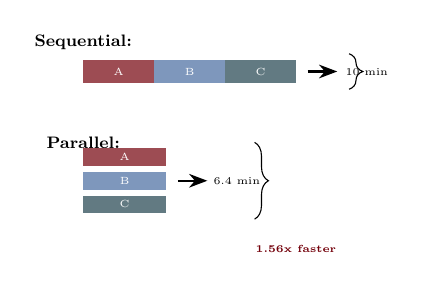
\begin{tikzpicture}[scale=0.75, transform shape]
                % Sequential execution
                \node[font=\footnotesize\bfseries] at (0,2.5) {Sequential:};
                \fill[UofSCGarnet!70] (0,1.8) rectangle (1.2,2.2);
                \fill[UofSCAtlantic!70] (1.2,1.8) rectangle (2.4,2.2);
                \fill[UofSCCongaree!70] (2.4,1.8) rectangle (3.6,2.2);
                \node[font=\tiny,white] at (0.6,2) {A};
                \node[font=\tiny,white] at (1.8,2) {B};
                \node[font=\tiny,white] at (3.0,2) {C};
                \draw[myarrow] (3.8,2) -- (4.3,2);
                \node[font=\tiny] at (4.8,2) {10 min};

                % Parallel execution
                \node[font=\footnotesize\bfseries] at (0,0.8) {Parallel:};
                \fill[UofSCGarnet!70] (0,0.4) rectangle (1.4,0.7);
                \fill[UofSCAtlantic!70] (0,0) rectangle (1.4,0.3);
                \fill[UofSCCongaree!70] (0,-0.4) rectangle (1.4,-0.1);
                \node[font=\tiny,white] at (0.7,0.55) {A};
                \node[font=\tiny,white] at (0.7,0.15) {B};
                \node[font=\tiny,white] at (0.7,-0.25) {C};
                \draw[myarrow] (1.6,0.15) -- (2.1,0.15);
                \node[font=\tiny] at (2.6,0.15) {6.4 min};

                % Speedup annotation
                \draw[decorate,decoration={brace,amplitude=5pt,mirror}] (4.5,1.7) -- (4.5,2.3);
                \draw[decorate,decoration={brace,amplitude=5pt,mirror}] (2.9,-0.5) -- (2.9,0.8);
                \node[font=\tiny\bfseries,UofSCGarnet] at (3.6,-1) {1.56x faster};
            \end{tikzpicture}
        \end{column}
    \end{columns}

    \note{Parallelization is one of the most impactful techniques in agentic coding. When tasks are independent, running them simultaneously saves substantial wall-clock time.}
\end{frame}

% ----------------------------------------------------------------------------
\begin{frame}{Performance Gains Across Task Types}
    \begin{columns}[T]
        \begin{column}{0.48\textwidth}
            \begin{block}{Research Phase Tasks}
                \textbf{40--50\% faster}
                \begin{itemize}
                    \item Literature review + codebase exploration
                    \item 8 min instead of 15 min
                \end{itemize}
            \end{block}

            \begin{block}{Code Analysis Tasks}
                \textbf{35--45\% faster}
                \begin{itemize}
                    \item Trace flow + search patterns + check docs
                    \item 12 min vs 20 min sequential
                \end{itemize}
            \end{block}
        \end{column}
        \begin{column}{0.48\textwidth}
            \begin{block}{Data Processing Tasks}
                \textbf{60--70\% faster}
                \begin{itemize}
                    \item Multiple parameter sweeps
                    \item 5 min instead of 45 min
                \end{itemize}
            \end{block}

            \begin{block}{Build \& Test}
                \textbf{30--40\% faster}
                \begin{itemize}
                    \item Lint + test + docs simultaneously
                    \item 3 min instead of 5 min
                \end{itemize}
            \end{block}
        \end{column}
    \end{columns}

    \vspace{0.3cm}
    \begin{center}
        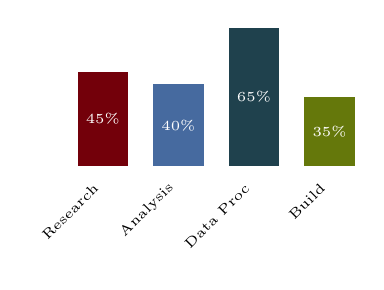
\begin{tikzpicture}[scale=0.8]
            % Bar chart
            \fill[UofSCGarnet] (0,0) rectangle (0.8,1.5);
            \fill[UofSCAtlantic] (1.2,0) rectangle (2,1.3);
            \fill[UofSCCongaree] (2.4,0) rectangle (3.2,2.2);
            \fill[UofSCHorseshoe] (3.6,0) rectangle (4.4,1.1);

            \node[font=\tiny,rotate=45,anchor=east] at (0.4,-0.2) {Research};
            \node[font=\tiny,rotate=45,anchor=east] at (1.6,-0.2) {Analysis};
            \node[font=\tiny,rotate=45,anchor=east] at (2.8,-0.2) {Data Proc};
            \node[font=\tiny,rotate=45,anchor=east] at (4,-0.2) {Build};

            \node[font=\tiny,white] at (0.4,0.75) {45\%};
            \node[font=\tiny,white] at (1.6,0.65) {40\%};
            \node[font=\tiny,white] at (2.8,1.1) {65\%};
            \node[font=\tiny,white] at (4,0.55) {35\%};
        \end{tikzpicture}
    \end{center}
\end{frame}

% ----------------------------------------------------------------------------
\begin{frame}{How Parallelization Improves Code Quality}
    \begin{columns}[T]
        \begin{column}{0.55\textwidth}
            \textbf{Multiple Perspectives}
            \begin{itemize}
                \item Agent 1: Performance focus
                \item Agent 2: Readability focus
                \item Agent 3: Maintainability focus
                \item Consensus emerges on best solution
            \end{itemize}

            \vspace{0.3cm}
            \textbf{Cross-Validation}
            \begin{itemize}
                \item 2/3 agents agree $\rightarrow$ likely correct
                \item Divergent results $\rightarrow$ investigate
                \item Reduces hallucination through consensus
            \end{itemize}

            \vspace{0.3cm}
            \textbf{Coverage Improvement}
            \begin{itemize}
                \item Agent A: Functionality tests
                \item Agent B: Edge case tests
                \item Agent C: Performance tests
                \item Result: 90\% more coverage
            \end{itemize}
        \end{column}
        \begin{column}{0.43\textwidth}
            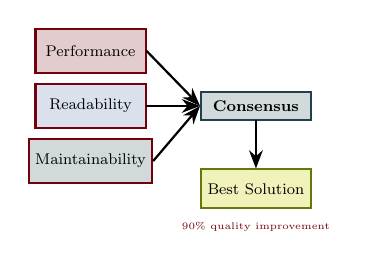
\begin{tikzpicture}[scale=0.7, transform shape]
                % Three agents
                \node[agentbox,fill=UofSCGarnet!20] (a1) at (0,3) {Performance};
                \node[agentbox,fill=UofSCAtlantic!20] (a2) at (0,2) {Readability};
                \node[agentbox,fill=UofSCCongaree!20] (a3) at (0,1) {Maintainability};

                % Convergence point
                \node[syncbox,minimum width=2cm] (sync) at (3,2) {Consensus};

                % Result
                \node[resultbox] (result) at (3,0.5) {Best Solution};

                % Arrows
                \draw[myarrow] (a1.east) -- (sync.west);
                \draw[myarrow] (a2.east) -- (sync.west);
                \draw[myarrow] (a3.east) -- (sync.west);
                \draw[myarrow] (sync.south) -- (result.north);

                % Annotation
                \node[font=\tiny,UofSCGarnet] at (3,-0.2) {90\% quality improvement};
            \end{tikzpicture}
        \end{column}
    \end{columns}
\end{frame}

% ----------------------------------------------------------------------------
\begin{frame}{Decision Matrix: Parallel vs Sequential}
    \begin{columns}[T]
        \begin{column}{0.48\textwidth}
            \begin{alertblock}{Use Parallel When:}
                \begin{itemize}
                    \item Tasks have NO data dependencies
                    \item Sequential time $>$ 10 minutes
                    \item Multiple perspectives improve quality
                    \item Budget for increased tokens
                    \item Minimal synchronization points
                \end{itemize}
            \end{alertblock}

            \begin{exampleblock}{Use Sequential When:}
                \begin{itemize}
                    \item Task B requires output from Task A
                    \item Sequential time $<$ 5 minutes
                    \item Token budget is constrained
                    \item Tasks are tightly coupled
                    \item Single agent has sufficient expertise
                \end{itemize}
            \end{exampleblock}
        \end{column}
        \begin{column}{0.48\textwidth}
            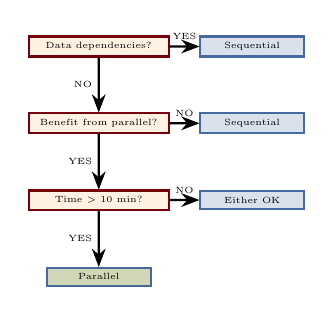
\begin{tikzpicture}[scale=0.65, transform shape,
                decision/.style={rectangle, draw=UofSCGarnet, thick, fill=UofSCSandstorm, text width=2.5cm, text centered, font=\tiny},
                outcome/.style={rectangle, draw=UofSCAtlantic, thick, fill=UofSCAtlantic!20, text width=1.8cm, text centered, font=\tiny}
            ]
                \node[decision] (d1) at (0,4) {Data dependencies?};
                \node[outcome] (seq1) at (3,4) {Sequential};
                \node[decision] (d2) at (0,2.5) {Benefit from parallel?};
                \node[outcome] (seq2) at (3,2.5) {Sequential};
                \node[decision] (d3) at (0,1) {Time $>$ 10 min?};
                \node[outcome] (either) at (3,1) {Either OK};
                \node[outcome,fill=UofSCHorseshoe!30] (par) at (0,-0.5) {Parallel};

                \draw[myarrow] (d1) -- node[above,font=\tiny]{YES} (seq1);
                \draw[myarrow] (d1) -- node[left,font=\tiny]{NO} (d2);
                \draw[myarrow] (d2) -- node[above,font=\tiny]{NO} (seq2);
                \draw[myarrow] (d2) -- node[left,font=\tiny]{YES} (d3);
                \draw[myarrow] (d3) -- node[above,font=\tiny]{NO} (either);
                \draw[myarrow] (d3) -- node[left,font=\tiny]{YES} (par);
            \end{tikzpicture}
        \end{column}
    \end{columns}
\end{frame}

% ----------------------------------------------------------------------------
\begin{frame}{Understanding the Token Cost of Parallelization}
    \begin{columns}[T]
        \begin{column}{0.48\textwidth}
            \textbf{Token Multiplication Factor}
            \begin{itemize}
                \item 1 agent: 10,000 tokens
                \item 3 parallel: $\sim$30,000 tokens
                \item 5 parallel: $\sim$50,000 tokens
            \end{itemize}

            \vspace{0.3cm}
            \textbf{Why Tokens Multiply}
            \begin{itemize}
                \item Each agent receives full context
                \item Independent reasoning (not shared)
                \item System prompts repeated
            \end{itemize}

            \vspace{0.3cm}
            \textbf{Mitigation Strategies}
            \begin{itemize}
                \item Use smaller models for parallel tasks
                \item Compress context for parallel agents
                \item Parallelize only critical path
            \end{itemize}
        \end{column}
        \begin{column}{0.48\textwidth}
            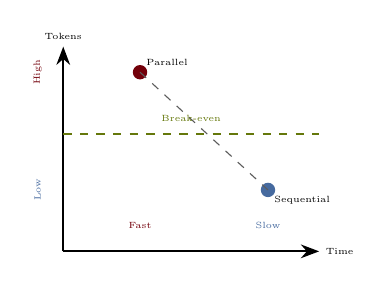
\begin{tikzpicture}[scale=0.65, transform shape]
                % Cost-benefit visualization
                \draw[timeline] (0,0) -- (5,0) node[right,font=\tiny]{Time};
                \draw[timeline] (0,0) -- (0,4) node[above,font=\tiny]{Tokens};

                % Sequential point
                \fill[UofSCAtlantic] (4,1.2) circle (4pt);
                \node[font=\tiny,below right] at (4,1.2) {Sequential};

                % Parallel point
                \fill[UofSCGarnet] (1.5,3.5) circle (4pt);
                \node[font=\tiny,above right] at (1.5,3.5) {Parallel};

                % Trade-off line
                \draw[dashed,UofSC70Black] (1.5,3.5) -- (4,1.2);

                % Annotations
                \node[font=\tiny,UofSCGarnet] at (1.5,0.5) {Fast};
                \node[font=\tiny,UofSCAtlantic] at (4,0.5) {Slow};
                \node[font=\tiny,UofSCGarnet,rotate=90] at (-0.5,3.5) {High};
                \node[font=\tiny,UofSCAtlantic,rotate=90] at (-0.5,1.2) {Low};

                % Decision zone
                \draw[thick,UofSCHorseshoe,dashed] (0,2.3) -- (5,2.3);
                \node[font=\tiny,UofSCHorseshoe] at (2.5,2.6) {Break-even};
            \end{tikzpicture}

            \vspace{0.3cm}
            \begin{block}{Cost-Benefit Rule}
                \footnotesize
                Worth it if: Time value $>$ Token cost
            \end{block}
        \end{column}
    \end{columns}
\end{frame}

% ----------------------------------------------------------------------------
\begin{frame}{Parallelization in Your Development Process}
    \begin{center}
        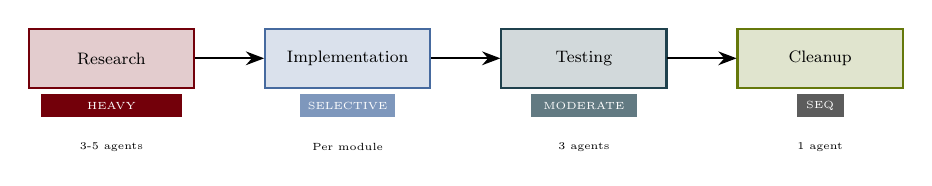
\begin{tikzpicture}[scale=0.75, transform shape]
            % Phase boxes
            \node[rectangle,draw=UofSCGarnet,thick,fill=UofSCGarnet!20,minimum width=2.8cm,minimum height=1cm] (research) at (0,0) {\footnotesize Research};
            \node[rectangle,draw=UofSCAtlantic,thick,fill=UofSCAtlantic!20,minimum width=2.8cm,minimum height=1cm] (impl) at (4,0) {\footnotesize Implementation};
            \node[rectangle,draw=UofSCCongaree,thick,fill=UofSCCongaree!20,minimum width=2.8cm,minimum height=1cm] (test) at (8,0) {\footnotesize Testing};
            \node[rectangle,draw=UofSCHorseshoe,thick,fill=UofSCHorseshoe!20,minimum width=2.8cm,minimum height=1cm] (clean) at (12,0) {\footnotesize Cleanup};

            % Parallelization intensity bars
            \fill[UofSCGarnet] (0-1.2,-1) rectangle (0+1.2,-0.6);
            \node[font=\tiny,white] at (0,-0.8) {HEAVY};

            \fill[UofSCAtlantic!70] (4-0.8,-1) rectangle (4+0.8,-0.6);
            \node[font=\tiny,white] at (4,-0.8) {SELECTIVE};

            \fill[UofSCCongaree!70] (8-0.9,-1) rectangle (8+0.9,-0.6);
            \node[font=\tiny,white] at (8,-0.8) {MODERATE};

            \fill[UofSC70Black] (12-0.4,-1) rectangle (12+0.4,-0.6);
            \node[font=\tiny,white] at (12,-0.8) {SEQ};

            % Arrows
            \draw[myarrow] (research.east) -- (impl.west);
            \draw[myarrow] (impl.east) -- (test.west);
            \draw[myarrow] (test.east) -- (clean.west);

            % Agent indicators
            \node[font=\tiny] at (0,-1.5) {3-5 agents};
            \node[font=\tiny] at (4,-1.5) {Per module};
            \node[font=\tiny] at (8,-1.5) {3 agents};
            \node[font=\tiny] at (12,-1.5) {1 agent};
        \end{tikzpicture}
    \end{center}

    \vspace{0.3cm}
    \begin{columns}[T]
        \begin{column}{0.48\textwidth}
            \begin{block}{Research Phase}
                \footnotesize
                Explore codebase + search literature + identify patterns (all simultaneously)
            \end{block}
        \end{column}
        \begin{column}{0.48\textwidth}
            \begin{block}{Review/Testing Phase}
                \footnotesize
                Different test suites in parallel; different linting rules simultaneously
            \end{block}
        \end{column}
    \end{columns}
\end{frame}

% ============================================================================
% SECTION 2: PARALLELIZATION FUNDAMENTALS
% ============================================================================
\section{Parallelization Fundamentals}

% ----------------------------------------------------------------------------
\begin{frame}{The Foundation: Task Independence}
    \begin{columns}[T]
        \begin{column}{0.55\textwidth}
            \textbf{Independent Tasks}
            \begin{itemize}
                \item Can run in any order, produce same result
                \item Agent A: Analyze performance
                \item Agent B: Check style compliance
                \item Agent C: Review security
                \item Order ABC, CAB, BCA $\rightarrow$ same result
            \end{itemize}

            \vspace{0.2cm}
            \textbf{Dependent Tasks}
            \begin{itemize}
                \item B requires A's output
                \item Agent A: Parse data $\rightarrow$ \texttt{parsed\_data}
                \item Agent B: Analyze \texttt{parsed\_data}
                \item Must run A first, then B
            \end{itemize}
        \end{column}
        \begin{column}{0.43\textwidth}
            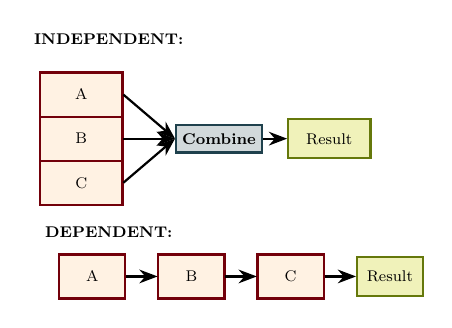
\begin{tikzpicture}[scale=0.7, transform shape]
                % Independent graph
                \node[font=\footnotesize\bfseries] at (0,4.5) {INDEPENDENT:};
                \node[agentbox,minimum width=1.5cm] (ia) at (-0.5,3.5) {A};
                \node[agentbox,minimum width=1.5cm] (ib) at (-0.5,2.7) {B};
                \node[agentbox,minimum width=1.5cm] (ic) at (-0.5,1.9) {C};
                \node[syncbox,minimum width=1.5cm] (icomb) at (2,2.7) {Combine};
                \node[resultbox,minimum width=1.5cm] (iresult) at (4,2.7) {Result};

                \draw[myarrow] (ia.east) -- (icomb.west);
                \draw[myarrow] (ib.east) -- (icomb.west);
                \draw[myarrow] (ic.east) -- (icomb.west);
                \draw[myarrow] (icomb.east) -- (iresult.west);

                % Dependent graph
                \node[font=\footnotesize\bfseries] at (0,1) {DEPENDENT:};
                \node[agentbox,minimum width=1.2cm] (da) at (-0.3,0.2) {A};
                \node[agentbox,minimum width=1.2cm] (db) at (1.5,0.2) {B};
                \node[agentbox,minimum width=1.2cm] (dc) at (3.3,0.2) {C};
                \node[resultbox,minimum width=1.2cm] (dresult) at (5.1,0.2) {Result};

                \draw[myarrow] (da.east) -- (db.west);
                \draw[myarrow] (db.east) -- (dc.west);
                \draw[myarrow] (dc.east) -- (dresult.west);
            \end{tikzpicture}
        \end{column}
    \end{columns}
\end{frame}

% ----------------------------------------------------------------------------
\begin{frame}{Dependency Graph Visualization}
    \begin{center}
        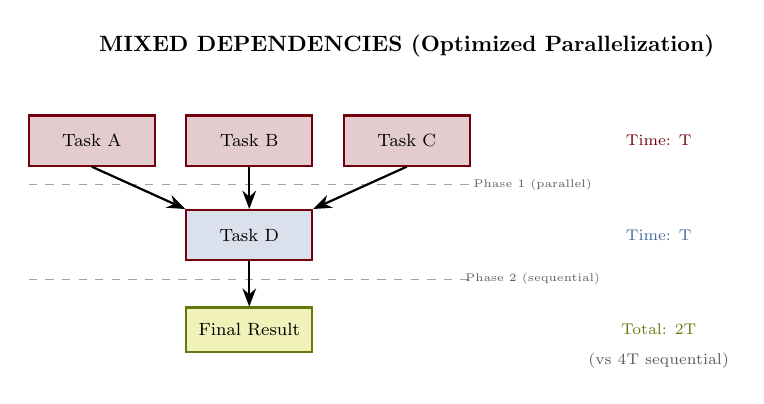
\begin{tikzpicture}[scale=0.8, transform shape]
            % Mixed dependency example
            \node[font=\bfseries] at (5,4.5) {MIXED DEPENDENCIES (Optimized Parallelization)};

            % Phase 1 - parallel
            \node[agentbox,fill=UofSCGarnet!20] (a) at (0,3) {Task A};
            \node[agentbox,fill=UofSCGarnet!20] (b) at (2.5,3) {Task B};
            \node[agentbox,fill=UofSCGarnet!20] (c) at (5,3) {Task C};

            % Phase 1 label
            \draw[dashed,UofSC50Black] (-1,2.3) -- (6,2.3);
            \node[font=\tiny,UofSC70Black] at (7,2.3) {Phase 1 (parallel)};

            % Phase 2 - depends on phase 1
            \node[agentbox,fill=UofSCAtlantic!20] (d) at (2.5,1.5) {Task D};

            % Phase 2 label
            \draw[dashed,UofSC50Black] (-1,0.8) -- (6,0.8);
            \node[font=\tiny,UofSC70Black] at (7,0.8) {Phase 2 (sequential)};

            % Result
            \node[resultbox] (result) at (2.5,0) {Final Result};

            % Arrows
            \draw[myarrow] (a.south) -- (d.north west);
            \draw[myarrow] (b.south) -- (d.north);
            \draw[myarrow] (c.south) -- (d.north east);
            \draw[myarrow] (d.south) -- (result.north);

            % Timing annotation
            \node[font=\scriptsize,UofSCGarnet] at (9,3) {Time: T};
            \node[font=\scriptsize,UofSCAtlantic] at (9,1.5) {Time: T};
            \node[font=\scriptsize,UofSCHorseshoe] at (9,0) {Total: 2T};
            \node[font=\scriptsize,UofSC70Black] at (9,-0.5) {(vs 4T sequential)};
        \end{tikzpicture}
    \end{center}

    \vspace{0.3cm}
    \begin{block}{Key Insight}
        You can parallelize tasks at the same ``level'' (with no edges between them). This often requires careful problem decomposition.
    \end{block}
\end{frame}

% ----------------------------------------------------------------------------
\begin{frame}{Synchronization Points}
    \begin{center}
        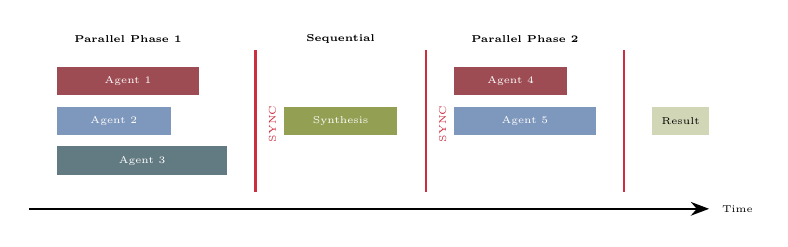
\begin{tikzpicture}[scale=0.72, transform shape]
            % Timeline
            \draw[timeline] (0,0) -- (12,0);
            \node[font=\tiny] at (12.5,0) {Time};

            % Phase 1 - Parallel
            \fill[UofSCGarnet!70] (0.5,2) rectangle (3,2.5);
            \fill[UofSCAtlantic!70] (0.5,1.3) rectangle (2.5,1.8);
            \fill[UofSCCongaree!70] (0.5,0.6) rectangle (3.5,1.1);

            \node[font=\tiny,white] at (1.75,2.25) {Agent 1};
            \node[font=\tiny,white] at (1.5,1.55) {Agent 2};
            \node[font=\tiny,white] at (2,0.85) {Agent 3};

            % Sync barrier 1
            \draw[thick,UofSCRose] (4,0.3) -- (4,2.8);
            \node[font=\tiny,UofSCRose,rotate=90] at (4.3,1.5) {SYNC};

            % Synthesis phase
            \fill[UofSCHorseshoe!70] (4.5,1.3) rectangle (6.5,1.8);
            \node[font=\tiny,white] at (5.5,1.55) {Synthesis};

            % Sync barrier 2
            \draw[thick,UofSCRose] (7,0.3) -- (7,2.8);
            \node[font=\tiny,UofSCRose,rotate=90] at (7.3,1.5) {SYNC};

            % Phase 2 - Parallel again
            \fill[UofSCGarnet!70] (7.5,2) rectangle (9.5,2.5);
            \fill[UofSCAtlantic!70] (7.5,1.3) rectangle (10,1.8);

            \node[font=\tiny,white] at (8.5,2.25) {Agent 4};
            \node[font=\tiny,white] at (8.75,1.55) {Agent 5};

            % Final sync
            \draw[thick,UofSCRose] (10.5,0.3) -- (10.5,2.8);

            % Result
            \fill[UofSCHorseshoe!30] (11,1.3) rectangle (12,1.8);
            \node[font=\tiny] at (11.5,1.55) {Result};

            % Labels
            \node[font=\tiny\bfseries] at (1.75,3) {Parallel Phase 1};
            \node[font=\tiny\bfseries] at (5.5,3) {Sequential};
            \node[font=\tiny\bfseries] at (8.75,3) {Parallel Phase 2};
        \end{tikzpicture}
    \end{center}

    \vspace{0.3cm}
    \begin{columns}[T]
        \begin{column}{0.32\textwidth}
            \begin{block}{Full Barrier}
                \footnotesize
                Wait for ALL agents before proceeding
            \end{block}
        \end{column}
        \begin{column}{0.32\textwidth}
            \begin{block}{Partial Barrier}
                \footnotesize
                Wait for ANY N agents (redundancy)
            \end{block}
        \end{column}
        \begin{column}{0.32\textwidth}
            \begin{block}{Timeout Barrier}
                \footnotesize
                Wait up to 5 min, proceed with results
            \end{block}
        \end{column}
    \end{columns}
\end{frame}

% ----------------------------------------------------------------------------
\begin{frame}{Batch Execution and Agent Lifecycle}
    \begin{center}
        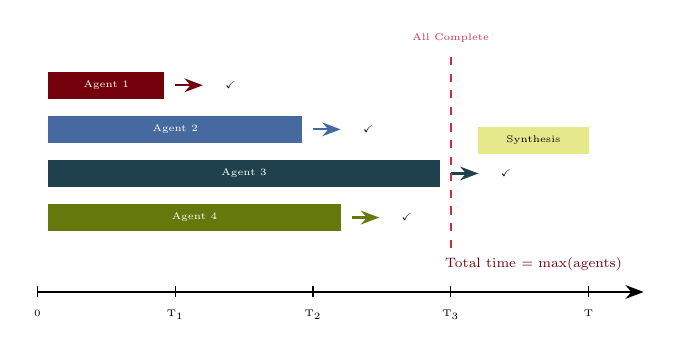
\begin{tikzpicture}[scale=0.7, transform shape]
            % Timeline axis
            \draw[timeline] (0,0) -- (11,0);
            \foreach \x/\l in {0/0,2.5/T$_1$,5/T$_2$,7.5/T$_3$,10/T} {
                \draw (\x,-0.1) -- (\x,0.1);
                \node[font=\tiny,below] at (\x,-0.2) {\l};
            }

            % Agent 1 - fast
            \fill[UofSCGarnet] (0.2,3.5) rectangle (2.3,4);
            \node[font=\tiny,white] at (1.25,3.75) {Agent 1};
            \draw[myarrow,UofSCGarnet] (2.5,3.75) -- (3,3.75);
            \node[font=\tiny] at (3.5,3.75) {\checkmark};

            % Agent 2 - medium
            \fill[UofSCAtlantic] (0.2,2.7) rectangle (4.8,3.2);
            \node[font=\tiny,white] at (2.5,2.95) {Agent 2};
            \draw[myarrow,UofSCAtlantic] (5,2.95) -- (5.5,2.95);
            \node[font=\tiny] at (6,2.95) {\checkmark};

            % Agent 3 - slow
            \fill[UofSCCongaree] (0.2,1.9) rectangle (7.3,2.4);
            \node[font=\tiny,white] at (3.75,2.15) {Agent 3};
            \draw[myarrow,UofSCCongaree] (7.5,2.15) -- (8,2.15);
            \node[font=\tiny] at (8.5,2.15) {\checkmark};

            % Agent 4 - medium
            \fill[UofSCHorseshoe] (0.2,1.1) rectangle (5.5,1.6);
            \node[font=\tiny,white] at (2.85,1.35) {Agent 4};
            \draw[myarrow,UofSCHorseshoe] (5.7,1.35) -- (6.2,1.35);
            \node[font=\tiny] at (6.7,1.35) {\checkmark};

            % Completion line
            \draw[thick,dashed,UofSCRose] (7.5,0.8) -- (7.5,4.3);
            \node[font=\tiny,UofSCRose] at (7.5,4.6) {All Complete};

            % Synthesis
            \fill[UofSCGrass!50] (8,2.5) rectangle (10,3);
            \node[font=\tiny] at (9,2.75) {Synthesis};

            % Annotations
            \node[font=\scriptsize,UofSCGarnet] at (9,0.5) {Total time = max(agents)};
        \end{tikzpicture}
    \end{center}

    \vspace{0.2cm}
    \begin{columns}[T]
        \begin{column}{0.48\textwidth}
            \textbf{Lifecycle Characteristics}
            \begin{itemize}
                \footnotesize
                \item All agents receive FULL context
                \item Agents don't communicate with each other
                \item Each agent has isolated workspace
                \item Results collected after completion
            \end{itemize}
        \end{column}
        \begin{column}{0.48\textwidth}
            \textbf{Maximum Parallelism}
            \begin{itemize}
                \footnotesize
                \item Claude Code: 10 concurrent agents
                \item Cursor: 8 concurrent agents
                \item Continue CLI: Unlimited (rate limited)
            \end{itemize}
        \end{column}
    \end{columns}
\end{frame}

% ----------------------------------------------------------------------------
\begin{frame}{Error Handling and Fault Tolerance}
    \begin{columns}[T]
        \begin{column}{0.48\textwidth}
            \textbf{Failure Modes}
            \begin{itemize}
                \item Agent timeout (30-60 min limit)
                \item Agent crash (OOM)
                \item Invalid output (malformed)
                \item Partial failure
            \end{itemize}

            \vspace{0.3cm}
            \textbf{Recovery Strategies}
            \begin{itemize}
                \item \textbf{Consensus}: 2/3 succeed $\rightarrow$ use majority
                \item \textbf{Redundancy}: Run 5 agents, need 4+ agree
                \item \textbf{Fallback}: Sequential retry if parallel fails
            \end{itemize}
        \end{column}
        \begin{column}{0.48\textwidth}
            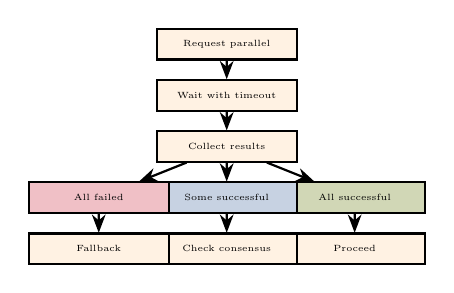
\begin{tikzpicture}[scale=0.65, transform shape,
                stepbox/.style={rectangle, draw=UofSCBlack, thick, fill=UofSCSandstorm, text width=2.5cm, text centered, font=\tiny, minimum height=0.6cm}
            ]
                \node[stepbox] (req) at (0,4) {Request parallel};
                \node[stepbox] (wait) at (0,3) {Wait with timeout};
                \node[stepbox] (collect) at (0,2) {Collect results};

                \node[stepbox,fill=UofSCHorseshoe!30] (allsuc) at (2.5,1) {All successful};
                \node[stepbox,fill=UofSCAtlantic!30] (some) at (0,1) {Some successful};
                \node[stepbox,fill=UofSCRose!30] (allfail) at (-2.5,1) {All failed};

                \node[stepbox] (proceed) at (2.5,0) {Proceed};
                \node[stepbox] (consensus) at (0,0) {Check consensus};
                \node[stepbox] (fallback) at (-2.5,0) {Fallback};

                \draw[myarrow] (req) -- (wait);
                \draw[myarrow] (wait) -- (collect);
                \draw[myarrow] (collect) -- (allsuc);
                \draw[myarrow] (collect) -- (some);
                \draw[myarrow] (collect) -- (allfail);
                \draw[myarrow] (allsuc) -- (proceed);
                \draw[myarrow] (some) -- (consensus);
                \draw[myarrow] (allfail) -- (fallback);
            \end{tikzpicture}
        \end{column}
    \end{columns}
\end{frame}

% ============================================================================
% SECTION 3: PARALLEL PATTERNS BY USE CASE
% ============================================================================
\section{Parallel Patterns by Use Case}

% ----------------------------------------------------------------------------
\begin{frame}{Pattern 1: Research \& Literature Review}
    \begin{columns}[T]
        \begin{column}{0.55\textwidth}
            \textbf{Three-Agent Research Breakdown}
            \begin{itemize}
                \item \textcolor{UofSCGarnet}{\textbf{Agent 1 - Codebase Explorer}}
                    \begin{itemize}
                        \footnotesize
                        \item File organization, module boundaries
                        \item Produces: Codebase map
                    \end{itemize}
                \item \textcolor{UofSCAtlantic}{\textbf{Agent 2 - Literature Searcher}}
                    \begin{itemize}
                        \footnotesize
                        \item Academic papers, official docs
                        \item Produces: Bibliography
                    \end{itemize}
                \item \textcolor{UofSCCongaree}{\textbf{Agent 3 - Pattern Identifier}}
                    \begin{itemize}
                        \footnotesize
                        \item Design patterns, similar solutions
                        \item Produces: Precedent list
                    \end{itemize}
            \end{itemize}

            \vspace{0.2cm}
            \textbf{Token Allocation}
            \begin{itemize}
                \footnotesize
                \item Per-agent: $\sim$2,000--3,000 tokens
                \item Total: $\sim$9,000 tokens (3 agents)
                \item Trade-off: +6,000 for better quality
            \end{itemize}
        \end{column}
        \begin{column}{0.43\textwidth}
            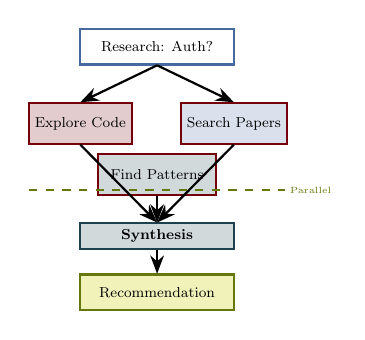
\begin{tikzpicture}[scale=0.65, transform shape]
                % Research task
                \node[processbox,minimum width=3cm] (task) at (1.5,4) {Research: Auth?};

                % Three parallel agents
                \node[agentbox,fill=UofSCGarnet!20,minimum width=2cm] (a1) at (0,2.5) {Explore Code};
                \node[agentbox,fill=UofSCAtlantic!20,minimum width=2cm] (a2) at (3,2.5) {Search Papers};
                \node[agentbox,fill=UofSCCongaree!20,minimum width=2.3cm] (a3) at (1.5,1.5) {Find Patterns};

                % Sync
                \node[syncbox,minimum width=3cm] (sync) at (1.5,0.3) {Synthesis};

                % Result
                \node[resultbox,minimum width=3cm] (result) at (1.5,-0.8) {Recommendation};

                % Arrows
                \draw[myarrow] (task.south) -- (a1.north);
                \draw[myarrow] (task.south) -- (a2.north);
                \draw[myarrow] (a1.south) -- (sync.north);
                \draw[myarrow] (a2.south) -- (sync.north);
                \draw[myarrow] (a3.south) -- (sync.north);
                \draw[myarrow] (sync.south) -- (result.north);

                % Parallel indicator
                \draw[thick,UofSCHorseshoe,dashed] (-1,1.2) -- (4,1.2);
                \node[font=\tiny,UofSCHorseshoe] at (4.5,1.2) {Parallel};
            \end{tikzpicture}
        \end{column}
    \end{columns}
\end{frame}

% ----------------------------------------------------------------------------
\begin{frame}{Pattern 2: Data Processing \& Experiments}
    \begin{center}
        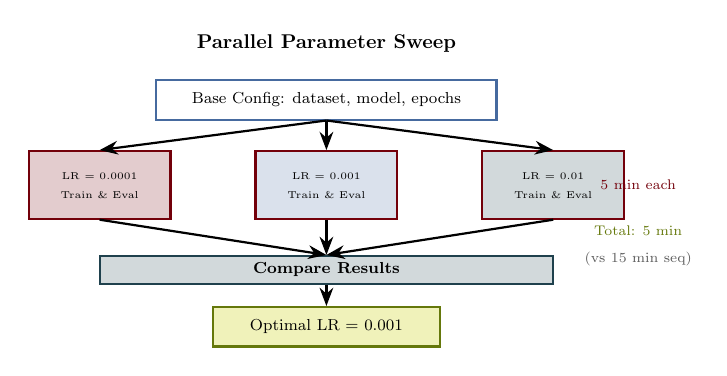
\begin{tikzpicture}[scale=0.72, transform shape]
            % Parameter sweep visualization
            \node[font=\bfseries] at (5.5,4) {Parallel Parameter Sweep};

            % Base config
            \node[processbox,minimum width=6cm] (base) at (5.5,3) {Base Config: dataset, model, epochs};

            % Three experiments
            \node[agentbox,fill=UofSCGarnet!20,minimum width=2.5cm,minimum height=1.2cm] (e1) at (1.5,1.5) {
                \begin{tabular}{c}
                    \tiny LR = 0.0001 \\
                    \tiny Train \& Eval
                \end{tabular}
            };
            \node[agentbox,fill=UofSCAtlantic!20,minimum width=2.5cm,minimum height=1.2cm] (e2) at (5.5,1.5) {
                \begin{tabular}{c}
                    \tiny LR = 0.001 \\
                    \tiny Train \& Eval
                \end{tabular}
            };
            \node[agentbox,fill=UofSCCongaree!20,minimum width=2.5cm,minimum height=1.2cm] (e3) at (9.5,1.5) {
                \begin{tabular}{c}
                    \tiny LR = 0.01 \\
                    \tiny Train \& Eval
                \end{tabular}
            };

            % Sync
            \node[syncbox,minimum width=8cm] (sync) at (5.5,0) {Compare Results};

            % Result
            \node[resultbox,minimum width=4cm] (result) at (5.5,-1) {Optimal LR = 0.001};

            % Arrows
            \draw[myarrow] (base.south) -- (e1.north);
            \draw[myarrow] (base.south) -- (e2.north);
            \draw[myarrow] (base.south) -- (e3.north);
            \draw[myarrow] (e1.south) -- (sync.north);
            \draw[myarrow] (e2.south) -- (sync.north);
            \draw[myarrow] (e3.south) -- (sync.north);
            \draw[myarrow] (sync.south) -- (result.north);

            % Timing
            \node[font=\scriptsize,UofSCGarnet] at (11,1.5) {5 min each};
            \node[font=\scriptsize,UofSCHorseshoe] at (11,0.7) {Total: 5 min};
            \node[font=\scriptsize,UofSC70Black] at (11,0.2) {(vs 15 min seq)};
        \end{tikzpicture}
    \end{center}

    \begin{block}{Speedup: 60--70\% Faster}
        \footnotesize
        Data processing tasks see the highest improvements because they're most parallelizable with minimal synchronization points.
    \end{block}
\end{frame}

% ----------------------------------------------------------------------------
\begin{frame}{Pattern 3: Code Analysis \& Debugging}
    \begin{columns}[T]
        \begin{column}{0.48\textwidth}
            \textbf{Three-Agent Code Review}
            \begin{itemize}
                \item \textcolor{UofSCGarnet}{\textbf{Correctness Reviewer}}
                    \begin{itemize}
                        \footnotesize
                        \item Logical errors, edge cases
                        \item Off-by-one errors
                    \end{itemize}
                \item \textcolor{UofSCAtlantic}{\textbf{Style Reviewer}}
                    \begin{itemize}
                        \footnotesize
                        \item Readability, naming
                        \item Structure improvements
                    \end{itemize}
                \item \textcolor{UofSCCongaree}{\textbf{Performance Reviewer}}
                    \begin{itemize}
                        \footnotesize
                        \item Efficiency, memory
                        \item Algorithmic improvements
                    \end{itemize}
            \end{itemize}

            \vspace{0.3cm}
            \textbf{Debugging Pattern}
            \begin{itemize}
                \footnotesize
                \item Agent 1: Trace data flow
                \item Agent 2: Search for similar bugs
                \item Agent 3: Review related tests
                \item Agent 4: Integrate and fix
            \end{itemize}
        \end{column}
        \begin{column}{0.48\textwidth}
            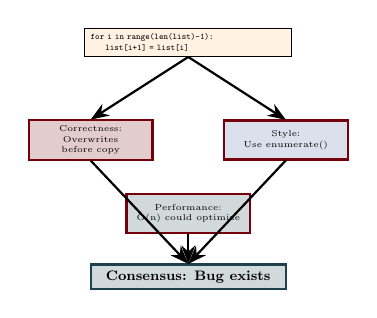
\begin{tikzpicture}[scale=0.62, transform shape]
                % Code snippet
                \node[rectangle,draw=UofSCBlack,fill=UofSCSandstorm,text width=4cm,font=\tiny\ttfamily] (code) at (2,4.5) {
                    for i in range(len(list)-1):\\
                    \hspace{0.3cm}list[i+1] = list[i]
                };

                % Three reviewers
                \node[agentbox,fill=UofSCGarnet!20,minimum width=2.5cm,text width=2.3cm,font=\tiny] (r1) at (0,2.5) {Correctness:\\Overwrites before copy};
                \node[agentbox,fill=UofSCAtlantic!20,minimum width=2.5cm,text width=2.3cm,font=\tiny] (r2) at (4,2.5) {Style:\\Use enumerate()};
                \node[agentbox,fill=UofSCCongaree!20,minimum width=2.5cm,text width=2.3cm,font=\tiny] (r3) at (2,1) {Performance:\\O(n) could optimize};

                % Consensus
                \node[syncbox,minimum width=4cm] (cons) at (2,-0.3) {Consensus: Bug exists};

                % Arrows
                \draw[myarrow] (code.south) -- (r1.north);
                \draw[myarrow] (code.south) -- (r2.north);
                \draw[myarrow] (r1.south) -- (cons.north);
                \draw[myarrow] (r2.south) -- (cons.north);
                \draw[myarrow] (r3.south) -- (cons.north);
            \end{tikzpicture}
        \end{column}
    \end{columns}
\end{frame}

% ----------------------------------------------------------------------------
\begin{frame}{Pattern 4: Build \& Test Parallelization}
    \begin{center}
        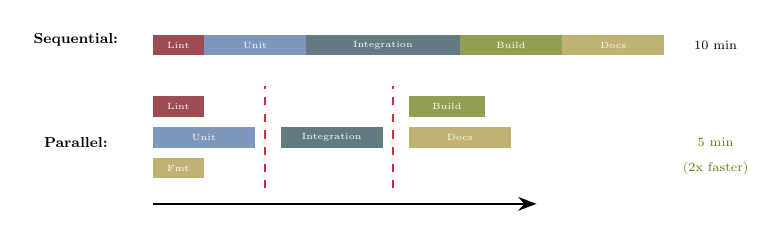
\begin{tikzpicture}[scale=0.65, transform shape]
            % Sequential comparison (top)
            \node[font=\footnotesize\bfseries] at (-1,3.5) {Sequential:};

            \fill[UofSCGarnet!70] (0.5,3.2) rectangle (1.5,3.6);
            \fill[UofSCAtlantic!70] (1.5,3.2) rectangle (3.5,3.6);
            \fill[UofSCCongaree!70] (3.5,3.2) rectangle (6.5,3.6);
            \fill[UofSCHorseshoe!70] (6.5,3.2) rectangle (8.5,3.6);
            \fill[UofSCHoneycomb!70] (8.5,3.2) rectangle (10.5,3.6);

            \node[font=\tiny,white] at (1,3.4) {Lint};
            \node[font=\tiny,white] at (2.5,3.4) {Unit};
            \node[font=\tiny,white] at (5,3.4) {Integration};
            \node[font=\tiny,white] at (7.5,3.4) {Build};
            \node[font=\tiny,white] at (9.5,3.4) {Docs};

            \node[font=\scriptsize] at (11.5,3.4) {10 min};

            % Parallel (bottom)
            \node[font=\footnotesize\bfseries] at (-1,1.5) {Parallel:};

            % Phase 1
            \fill[UofSCGarnet!70] (0.5,2) rectangle (1.5,2.4);
            \fill[UofSCAtlantic!70] (0.5,1.4) rectangle (2.5,1.8);
            \fill[UofSCHoneycomb!70] (0.5,0.8) rectangle (1.5,1.2);

            \node[font=\tiny,white] at (1,2.2) {Lint};
            \node[font=\tiny,white] at (1.5,1.6) {Unit};
            \node[font=\tiny,white] at (1,1) {Fmt};

            % Sync line
            \draw[thick,dashed,UofSCRose] (2.7,0.6) -- (2.7,2.6);

            % Phase 2
            \fill[UofSCCongaree!70] (3,1.4) rectangle (5,1.8);
            \node[font=\tiny,white] at (4,1.6) {Integration};

            % Sync line
            \draw[thick,dashed,UofSCRose] (5.2,0.6) -- (5.2,2.6);

            % Phase 3
            \fill[UofSCHorseshoe!70] (5.5,2) rectangle (7,2.4);
            \fill[UofSCHoneycomb!70] (5.5,1.4) rectangle (7.5,1.8);

            \node[font=\tiny,white] at (6.25,2.2) {Build};
            \node[font=\tiny,white] at (6.5,1.6) {Docs};

            \node[font=\scriptsize,UofSCHorseshoe] at (11.5,1.5) {5 min};
            \node[font=\scriptsize,UofSCHorseshoe] at (11.5,1) {(2x faster)};

            % Timeline
            \draw[timeline] (0.5,0.3) -- (8,0.3);
        \end{tikzpicture}
    \end{center}

    \vspace{0.3cm}
    \begin{columns}[T]
        \begin{column}{0.32\textwidth}
            \begin{block}{Phase 1}
                \footnotesize
                Lint, Unit Tests, Format (parallel)
            \end{block}
        \end{column}
        \begin{column}{0.32\textwidth}
            \begin{block}{Phase 2}
                \footnotesize
                Integration Tests (after Phase 1)
            \end{block}
        \end{column}
        \begin{column}{0.32\textwidth}
            \begin{block}{Phase 3}
                \footnotesize
                Build + Docs (parallel)
            \end{block}
        \end{column}
    \end{columns}
\end{frame}

% ----------------------------------------------------------------------------
\begin{frame}{Pattern 5: Content Generation}
    \begin{center}
        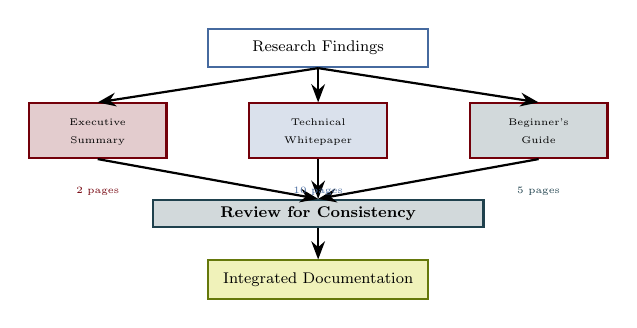
\begin{tikzpicture}[scale=0.7, transform shape]
            % Input
            \node[processbox,minimum width=4cm] (input) at (4,3.5) {Research Findings};

            % Parallel generation
            \node[agentbox,fill=UofSCGarnet!20,minimum width=2.5cm,minimum height=1cm] (g1) at (0,2) {
                \begin{tabular}{c}
                    \tiny Executive \\
                    \tiny Summary
                \end{tabular}
            };
            \node[agentbox,fill=UofSCAtlantic!20,minimum width=2.5cm,minimum height=1cm] (g2) at (4,2) {
                \begin{tabular}{c}
                    \tiny Technical \\
                    \tiny Whitepaper
                \end{tabular}
            };
            \node[agentbox,fill=UofSCCongaree!20,minimum width=2.5cm,minimum height=1cm] (g3) at (8,2) {
                \begin{tabular}{c}
                    \tiny Beginner's \\
                    \tiny Guide
                \end{tabular}
            };

            % Sync
            \node[syncbox,minimum width=6cm] (sync) at (4,0.5) {Review for Consistency};

            % Result
            \node[resultbox,minimum width=4cm] (result) at (4,-0.7) {Integrated Documentation};

            % Arrows
            \draw[myarrow] (input.south) -- (g1.north);
            \draw[myarrow] (input.south) -- (g2.north);
            \draw[myarrow] (input.south) -- (g3.north);
            \draw[myarrow] (g1.south) -- (sync.north);
            \draw[myarrow] (g2.south) -- (sync.north);
            \draw[myarrow] (g3.south) -- (sync.north);
            \draw[myarrow] (sync.south) -- (result.north);

            % Annotations
            \node[font=\tiny,UofSCGarnet] at (0,0.9) {2 pages};
            \node[font=\tiny,UofSCAtlantic] at (4,0.9) {10 pages};
            \node[font=\tiny,UofSCCongaree] at (8,0.9) {5 pages};
        \end{tikzpicture}
    \end{center}

    \begin{block}{Use Case}
        \footnotesize
        Generate different content pieces from the same source material in parallel. Each piece is independent---beginner's guide doesn't depend on technical whitepaper.
    \end{block}
\end{frame}

% ============================================================================
% SECTION 4: CLAUDE CODE DEEP DIVE
% ============================================================================
\section{Claude Code Parallelization}

% ----------------------------------------------------------------------------
\begin{frame}{Explicit Parallel Request Syntax}
    \begin{columns}[T]
        \begin{column}{0.48\textwidth}
            \textbf{Magic Keywords}
            \begin{itemize}
                \item ``in parallel''
                \item ``simultaneously''
                \item ``concurrently''
                \item ``at the same time''
            \end{itemize}

            \vspace{0.3cm}
            \textbf{Basic Syntax}
            \begin{lstlisting}[style=prompt]
Run these tasks in parallel:
1. [Task A description]
2. [Task B description]
3. [Task C description]

After completion, [synthesis]
            \end{lstlisting}
        \end{column}
        \begin{column}{0.48\textwidth}
            \textbf{Good vs Poor Requests}

            \begin{alertblock}{Poor (Ambiguous)}
                \footnotesize
                ``Explore the code. Search for papers. Find patterns.''
            \end{alertblock}

            \begin{exampleblock}{Good (Explicit)}
                \footnotesize
                ``Run three agents in parallel:
                \begin{enumerate}
                    \item Explore the codebase structure
                    \item Search for relevant papers
                    \item Find similar implementations
                \end{enumerate}
                Then combine findings.''
            \end{exampleblock}
        \end{column}
    \end{columns}
\end{frame}

% ----------------------------------------------------------------------------
\begin{frame}{Maximum Concurrent Agents and Scaling}
    \begin{columns}[T]
        \begin{column}{0.48\textwidth}
            \textbf{Maximum Parallel Agents: 10}

            \vspace{0.2cm}
            \begin{tabular}{lc}
                \toprule
                \textbf{Use Case} & \textbf{Recommended} \\
                \midrule
                Research & 3--5 agents \\
                Data processing & 5--10 agents \\
                Code analysis & 3--4 agents \\
                Build/testing & 5--8 agents \\
                \bottomrule
            \end{tabular}

            \vspace{0.3cm}
            \textbf{Resource Implications}
            \begin{itemize}
                \footnotesize
                \item 1 agent: $\sim$500MB memory
                \item 5 agents: $\sim$2.5GB memory
                \item 10 agents: $\sim$5GB memory
            \end{itemize}
        \end{column}
        \begin{column}{0.48\textwidth}
            \textbf{Beyond 10: Batching Strategy}

            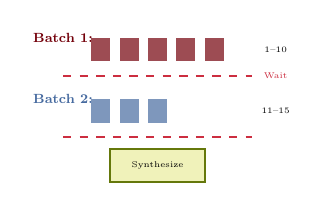
\begin{tikzpicture}[scale=0.6, transform shape]
                % Batch 1
                \node[font=\footnotesize\bfseries,UofSCGarnet] at (0,3) {Batch 1:};
                \foreach \x in {1,...,5} {
                    \fill[UofSCGarnet!70] (\x*0.6,2.5) rectangle (\x*0.6+0.4,3);
                }
                \node[font=\tiny] at (4.5,2.75) {1--10};

                % Sync
                \draw[thick,dashed,UofSCRose] (0,2.2) -- (4,2.2);
                \node[font=\tiny,UofSCRose] at (4.5,2.2) {Wait};

                % Batch 2
                \node[font=\footnotesize\bfseries,UofSCAtlantic] at (0,1.7) {Batch 2:};
                \foreach \x in {1,...,3} {
                    \fill[UofSCAtlantic!70] (\x*0.6,1.2) rectangle (\x*0.6+0.4,1.7);
                }
                \node[font=\tiny] at (4.5,1.45) {11--15};

                % Sync
                \draw[thick,dashed,UofSCRose] (0,0.9) -- (4,0.9);

                % Synthesis
                \node[resultbox,minimum width=2cm] at (2,0.3) {\tiny Synthesize};
            \end{tikzpicture}

            \vspace{0.2cm}
            \begin{block}{Token Formula}
                \footnotesize
                N agents $\approx$ N $\times$ baseline tokens
            \end{block}
        \end{column}
    \end{columns}
\end{frame}

% ----------------------------------------------------------------------------
\begin{frame}{The \texttt{run\_in\_background} Parameter}
    \begin{columns}[T]
        \begin{column}{0.55\textwidth}
            \textbf{When to Use Background Execution}
            \begin{itemize}
                \item Long data processing ($>$ 10 minutes)
                \item Extensive experimentation
                \item Building large projects
                \item Running full test suites
            \end{itemize}

            \vspace{0.2cm}
            \textbf{When NOT to Use}
            \begin{itemize}
                \item Tasks under 5 minutes
                \item Tasks needed for next step
                \item Interactive debugging
            \end{itemize}

            \vspace{0.2cm}
            \begin{block}{Pattern}
                \footnotesize
                Start long task in background $\rightarrow$ Do other work $\rightarrow$ Retrieve results $\rightarrow$ Synthesize
            \end{block}
        \end{column}
        \begin{column}{0.43\textwidth}
            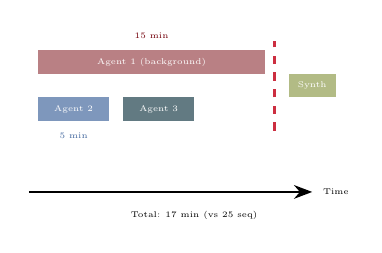
\begin{tikzpicture}[scale=0.6, transform shape]
                % Timeline
                \draw[timeline] (0,0) -- (6,0);
                \node[font=\tiny] at (6.5,0) {Time};

                % Background task (long)
                \fill[UofSCGarnet!50] (0.2,2.5) rectangle (5,3);
                \node[font=\tiny,white] at (2.6,2.75) {Agent 1 (background)};

                % Foreground tasks
                \fill[UofSCAtlantic!70] (0.2,1.5) rectangle (1.7,2);
                \node[font=\tiny,white] at (0.95,1.75) {Agent 2};

                \fill[UofSCCongaree!70] (2,1.5) rectangle (3.5,2);
                \node[font=\tiny,white] at (2.75,1.75) {Agent 3};

                % Sync and synthesis
                \draw[thick,dashed,UofSCRose] (5.2,1.3) -- (5.2,3.2);

                \fill[UofSCHorseshoe!50] (5.5,2) rectangle (6.5,2.5);
                \node[font=\tiny,white] at (6,2.25) {Synth};

                % Annotations
                \node[font=\tiny,UofSCGarnet] at (2.6,3.3) {15 min};
                \node[font=\tiny,UofSCAtlantic] at (0.95,1.2) {5 min};
                \node[font=\tiny] at (3.5,-0.5) {Total: 17 min (vs 25 seq)};
            \end{tikzpicture}
        \end{column}
    \end{columns}
\end{frame}

% ----------------------------------------------------------------------------
\begin{frame}{Ready-to-Use Prompt Templates}
    \begin{columns}[T]
        \begin{column}{0.48\textwidth}
            \begin{block}{Template 1: Research}
                \scriptsize
                ``Run 3 agents in parallel:
                \begin{itemize}
                    \item Agent 1 - Codebase Explorer
                    \item Agent 2 - Literature Searcher
                    \item Agent 3 - Pattern Researcher
                \end{itemize}
                After all complete, synthesize into report.''
            \end{block}

            \begin{block}{Template 2: Code Review}
                \scriptsize
                ``Review from 3 perspectives:
                \begin{itemize}
                    \item Agent 1 - Correctness
                    \item Agent 2 - Style
                    \item Agent 3 - Performance
                \end{itemize}
                Consensus: Issues 2+ agree on?''
            \end{block}
        \end{column}
        \begin{column}{0.48\textwidth}
            \begin{block}{Template 3: Experiments}
                \scriptsize
                ``Run experiments in parallel:
                \begin{itemize}
                    \item Agent 1: param=value1
                    \item Agent 2: param=value2
                    \item Agent 3: param=value3
                \end{itemize}
                After all, compare and identify optimal.''
            \end{block}

            \begin{block}{Template 4: Documentation}
                \scriptsize
                ``Generate docs in 3 formats:
                \begin{itemize}
                    \item Agent 1: Executive summary
                    \item Agent 2: Technical guide
                    \item Agent 3: API reference
                \end{itemize}
                Combine into integrated package.''
            \end{block}
        \end{column}
    \end{columns}
\end{frame}

% ============================================================================
% SECTION 5: BEST PRACTICES
% ============================================================================
\section{Best Practices}

% ----------------------------------------------------------------------------
\begin{frame}{Independence Requirements}
    \begin{columns}[T]
        \begin{column}{0.48\textwidth}
            \textbf{Independence Checklist}
            \begin{itemize}
                \item[$\square$] Task A's output NOT required by Task B
                \item[$\square$] Task B's output NOT required by Task A
                \item[$\square$] Both don't modify same files
                \item[$\square$] Order of execution doesn't matter
                \item[$\square$] Results can be combined without conflicts
            \end{itemize}

            \vspace{0.2cm}
            \textbf{All TRUE $\rightarrow$ Can parallelize}
        \end{column}
        \begin{column}{0.48\textwidth}
            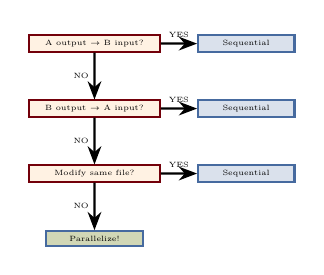
\begin{tikzpicture}[scale=0.55, transform shape,
                decision/.style={rectangle, draw=UofSCGarnet, thick, fill=UofSCSandstorm, text width=2.8cm, text centered, font=\tiny},
                outcome/.style={rectangle, draw=UofSCAtlantic, thick, fill=UofSCAtlantic!20, text width=2cm, text centered, font=\tiny}
            ]
                \node[decision] (d1) at (0,4) {A output $\rightarrow$ B input?};
                \node[outcome] (seq1) at (3.5,4) {Sequential};

                \node[decision] (d2) at (0,2.5) {B output $\rightarrow$ A input?};
                \node[outcome] (seq2) at (3.5,2.5) {Sequential};

                \node[decision] (d3) at (0,1) {Modify same file?};
                \node[outcome] (seq3) at (3.5,1) {Sequential};

                \node[outcome,fill=UofSCHorseshoe!30] (par) at (0,-0.5) {Parallelize!};

                \draw[myarrow] (d1) -- node[above,font=\tiny]{YES} (seq1);
                \draw[myarrow] (d1) -- node[left,font=\tiny]{NO} (d2);
                \draw[myarrow] (d2) -- node[above,font=\tiny]{YES} (seq2);
                \draw[myarrow] (d2) -- node[left,font=\tiny]{NO} (d3);
                \draw[myarrow] (d3) -- node[above,font=\tiny]{YES} (seq3);
                \draw[myarrow] (d3) -- node[left,font=\tiny]{NO} (par);
            \end{tikzpicture}
        \end{column}
    \end{columns}
\end{frame}

% ----------------------------------------------------------------------------
\begin{frame}{Specificity for Each Agent}
    \begin{columns}[T]
        \begin{column}{0.48\textwidth}
            \textbf{Good Role Naming}

            \begin{alertblock}{Vague}
                \footnotesize
                Agent 1, Agent 2, Agent 3
            \end{alertblock}

            \begin{exampleblock}{Specific}
                \footnotesize
                \begin{itemize}
                    \item Agent 1 - Correctness Reviewer
                    \item Agent 2 - Performance Analyzer
                    \item Agent 3 - Security Auditor
                \end{itemize}
            \end{exampleblock}
        \end{column}
        \begin{column}{0.48\textwidth}
            \textbf{Clear Task Instructions}

            \begin{alertblock}{Vague}
                \footnotesize
                ``Analyze this code''
            \end{alertblock}

            \begin{exampleblock}{Specific}
                \footnotesize
                ``Review this code for security vulnerabilities. Look for SQL injection, buffer overflows, privilege escalation. Provide specific code locations and severity levels.''
            \end{exampleblock}
        \end{column}
    \end{columns}

    \vspace{0.3cm}
    \begin{block}{Output Specification}
        \footnotesize
        Always specify expected output format (e.g., JSON, structured list, specific metrics).
    \end{block}
\end{frame}

% ----------------------------------------------------------------------------
\begin{frame}{Collecting and Synthesizing Results}
    \begin{columns}[T]
        \begin{column}{0.48\textwidth}
            \textbf{Synthesis Approaches}
            \begin{itemize}
                \item \textbf{MERGE}: Combine into single output
                \item \textbf{CONSENSUS}: Look for agreement
                \item \textbf{COMPARE}: Highlight differences
                \item \textbf{RANK}: Order by importance
            \end{itemize}

            \vspace{0.3cm}
            \textbf{Handling Contradictions}
            \begin{itemize}
                \footnotesize
                \item If Agent 1 says issue, Agent 2 says not
                \item Compare their reasoning
                \item Determine who is more likely correct
            \end{itemize}
        \end{column}
        \begin{column}{0.48\textwidth}
            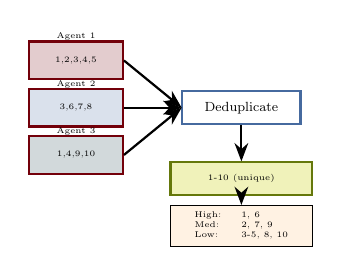
\begin{tikzpicture}[scale=0.6, transform shape]
                % Agent outputs
                \node[agentbox,fill=UofSCGarnet!20,minimum width=2cm,font=\tiny] (a1) at (0,3) {1,2,3,4,5};
                \node[agentbox,fill=UofSCAtlantic!20,minimum width=2cm,font=\tiny] (a2) at (0,2) {3,6,7,8};
                \node[agentbox,fill=UofSCCongaree!20,minimum width=2cm,font=\tiny] (a3) at (0,1) {1,4,9,10};

                \node[font=\tiny] at (0,3.5) {Agent 1};
                \node[font=\tiny] at (0,2.5) {Agent 2};
                \node[font=\tiny] at (0,1.5) {Agent 3};

                % Deduplication
                \node[processbox,minimum width=2.5cm] (dedup) at (3.5,2) {Deduplicate};

                % Unique findings
                \node[resultbox,minimum width=3cm,font=\tiny] (unique) at (3.5,0.5) {1-10 (unique)};

                % Categorization
                \node[rectangle,draw=UofSCBlack,minimum width=3cm,font=\tiny,fill=UofSCSandstorm] (cat) at (3.5,-0.5) {
                    \begin{tabular}{ll}
                        High: & 1, 6 \\
                        Med: & 2, 7, 9 \\
                        Low: & 3-5, 8, 10
                    \end{tabular}
                };

                \draw[myarrow] (a1.east) -- (dedup.west);
                \draw[myarrow] (a2.east) -- (dedup.west);
                \draw[myarrow] (a3.east) -- (dedup.west);
                \draw[myarrow] (dedup.south) -- (unique.north);
                \draw[myarrow] (unique.south) -- (cat.north);
            \end{tikzpicture}
        \end{column}
    \end{columns}
\end{frame}

% ----------------------------------------------------------------------------
\begin{frame}{Token Usage Monitoring}
    \begin{columns}[T]
        \begin{column}{0.48\textwidth}
            \textbf{Token Cost Model}
            \begin{itemize}
                \item Single agent: 3,000 tokens
                \item 3 parallel agents: $\sim$9,000 tokens
                \item Cost multiplier: 3x
            \end{itemize}

            \vspace{0.2cm}
            \textbf{Cost-Benefit Analysis}
            \begin{itemize}
                \footnotesize
                \item Extra tokens: 6,000
                \item Time saved: 5 minutes
                \item Worth it if: time value $>$ token cost
            \end{itemize}

            \vspace{0.2cm}
            \textbf{Optimization Techniques}
            \begin{itemize}
                \footnotesize
                \item Context compression
                \item Focus narrowing
                \item Smaller models for parallel
                \item Result deduplication
            \end{itemize}
        \end{column}
        \begin{column}{0.48\textwidth}
            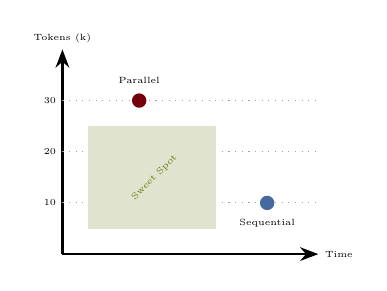
\begin{tikzpicture}[scale=0.65, transform shape]
                % Axes
                \draw[timeline] (0,0) -- (5,0) node[right,font=\tiny]{Time};
                \draw[timeline] (0,0) -- (0,4) node[above,font=\tiny]{Tokens (k)};

                % Grid
                \draw[UofSC50Black,dotted] (0,1) -- (5,1);
                \draw[UofSC50Black,dotted] (0,2) -- (5,2);
                \draw[UofSC50Black,dotted] (0,3) -- (5,3);

                % Labels
                \node[font=\tiny,left] at (0,1) {10};
                \node[font=\tiny,left] at (0,2) {20};
                \node[font=\tiny,left] at (0,3) {30};

                % Points
                \fill[UofSCAtlantic] (4,1) circle (4pt);
                \node[font=\tiny,below] at (4,0.8) {Sequential};

                \fill[UofSCGarnet] (1.5,3) circle (4pt);
                \node[font=\tiny,above] at (1.5,3.2) {Parallel};

                % Trade-off region
                \fill[UofSCHorseshoe!20] (0.5,0.5) rectangle (3,2.5);
                \node[font=\tiny,UofSCHorseshoe,rotate=45] at (1.8,1.5) {Sweet Spot};
            \end{tikzpicture}

            \vspace{0.2cm}
            \begin{block}{ROI Formula}
                \footnotesize
                ROI = Time Value - Token Cost \\
                Positive = Worth parallelizing
            \end{block}
        \end{column}
    \end{columns}
\end{frame}

% ============================================================================
% SECTION 6: ADVANCED TOPICS
% ============================================================================
\section{Advanced Topics}

% ----------------------------------------------------------------------------
\begin{frame}{Handling Large-Scale Parallelization}
    \begin{columns}[T]
        \begin{column}{0.48\textwidth}
            \textbf{When You Need $>$ 10 Agents}
            \begin{itemize}
                \item Large experiments (many parameters)
                \item Big data processing (multiple datasets)
                \item Comprehensive code analysis
                \item Extensive testing
            \end{itemize}

            \vspace{0.2cm}
            \textbf{Batching Strategy}
            \begin{itemize}
                \footnotesize
                \item Need 25 agents? Use 3 batches
                \item Batch 1: Agents 1--10
                \item Batch 2: Agents 11--20
                \item Batch 3: Agents 21--25
                \item Final: Combine all results
            \end{itemize}
        \end{column}
        \begin{column}{0.48\textwidth}
            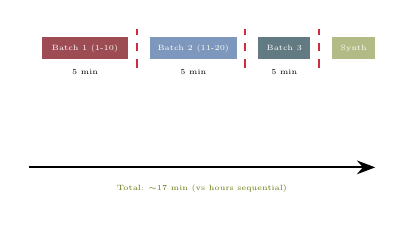
\begin{tikzpicture}[scale=0.55, transform shape]
                % Timeline
                \draw[timeline] (0,0) -- (8,0);

                % Batch 1
                \fill[UofSCGarnet!70] (0.3,2.5) rectangle (2.3,3);
                \node[font=\tiny,white] at (1.3,2.75) {Batch 1 (1-10)};

                % Collect 1
                \draw[thick,dashed,UofSCRose] (2.5,2.3) -- (2.5,3.2);

                % Batch 2
                \fill[UofSCAtlantic!70] (2.8,2.5) rectangle (4.8,3);
                \node[font=\tiny,white] at (3.8,2.75) {Batch 2 (11-20)};

                % Collect 2
                \draw[thick,dashed,UofSCRose] (5,2.3) -- (5,3.2);

                % Batch 3
                \fill[UofSCCongaree!70] (5.3,2.5) rectangle (6.5,3);
                \node[font=\tiny,white] at (5.9,2.75) {Batch 3};

                % Final sync
                \draw[thick,dashed,UofSCRose] (6.7,2.3) -- (6.7,3.2);

                % Synthesis
                \fill[UofSCHorseshoe!50] (7,2.5) rectangle (8,3);
                \node[font=\tiny,white] at (7.5,2.75) {Synth};

                % Time labels
                \node[font=\tiny] at (1.3,2.2) {5 min};
                \node[font=\tiny] at (3.8,2.2) {5 min};
                \node[font=\tiny] at (5.9,2.2) {5 min};

                % Annotation
                \node[font=\tiny,UofSCHorseshoe] at (4,-0.5) {Total: $\sim$17 min (vs hours sequential)};
            \end{tikzpicture}
        \end{column}
    \end{columns}

    \vspace{0.3cm}
    \begin{alertblock}{Resource Consideration}
        \footnotesize
        Running 10 concurrent agents is resource-intensive. Space agents across batches rather than cramming 20 into 2 batches.
    \end{alertblock}
\end{frame}

% ----------------------------------------------------------------------------
\begin{frame}{Error Recovery and Fault Tolerance}
    \begin{columns}[T]
        \begin{column}{0.48\textwidth}
            \textbf{Fault Tolerance Levels}
            \begin{itemize}
                \item \textbf{Level 1 (NONE)}: 1 fails $\rightarrow$ task fails
                \item \textbf{Level 2 (PARTIAL)}: Use results from others
                \item \textbf{Level 3 (FULL)}: Retry or use backup
            \end{itemize}

            \vspace{0.2cm}
            \textbf{Redundancy Pattern}
            \begin{itemize}
                \footnotesize
                \item N=1: No tolerance
                \item N=3: Can continue if 1 fails
                \item N=5: Can tolerate 2 failures
            \end{itemize}

            \vspace{0.2cm}
            \textbf{Fallback Strategies}
            \begin{itemize}
                \footnotesize
                \item Retry parallel with timeout extension
                \item Run sequential version
                \item Use last known good results
                \item Skip task, continue with others
            \end{itemize}
        \end{column}
        \begin{column}{0.48\textwidth}
            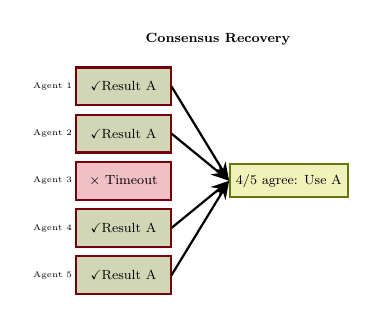
\begin{tikzpicture}[scale=0.6, transform shape]
                % Consensus example
                \node[font=\footnotesize\bfseries] at (2,4) {Consensus Recovery};

                \node[agentbox,fill=UofSCHorseshoe!30,minimum width=2cm] (a1) at (0,3) {\checkmark Result A};
                \node[agentbox,fill=UofSCHorseshoe!30,minimum width=2cm] (a2) at (0,2) {\checkmark Result A};
                \node[agentbox,fill=UofSCRose!30,minimum width=2cm] (a3) at (0,1) {$\times$ Timeout};
                \node[agentbox,fill=UofSCHorseshoe!30,minimum width=2cm] (a4) at (0,0) {\checkmark Result A};
                \node[agentbox,fill=UofSCHorseshoe!30,minimum width=2cm] (a5) at (0,-1) {\checkmark Result A};

                \node[font=\tiny] at (-1.5,3) {Agent 1};
                \node[font=\tiny] at (-1.5,2) {Agent 2};
                \node[font=\tiny] at (-1.5,1) {Agent 3};
                \node[font=\tiny] at (-1.5,0) {Agent 4};
                \node[font=\tiny] at (-1.5,-1) {Agent 5};

                % Result
                \node[resultbox,minimum width=2.5cm] (result) at (3.5,1) {4/5 agree: Use A};

                \draw[myarrow] (a1.east) -- (result.west);
                \draw[myarrow] (a2.east) -- (result.west);
                \draw[myarrow] (a4.east) -- (result.west);
                \draw[myarrow] (a5.east) -- (result.west);
            \end{tikzpicture}
        \end{column}
    \end{columns}
\end{frame}

% ============================================================================
% SECTION 7: SUMMARY
% ============================================================================
\section{Summary and Key Takeaways}

% ----------------------------------------------------------------------------
\begin{frame}{Key Takeaways}
    \begin{columns}[T]
        \begin{column}{0.48\textwidth}
            \begin{block}{1. Independence is Everything}
                \footnotesize
                Parallelize only truly independent tasks. If B needs A's output, must run sequentially.
            \end{block}

            \begin{block}{2. Explicit is Better}
                \footnotesize
                Use clear ``run in parallel'' language. Give each agent specific role and instructions.
            \end{block}

            \begin{block}{3. Cost-Benefit Analysis}
                \footnotesize
                3x tokens for 3 agents. Worth it when time saved $>$ token cost.
            \end{block}
        \end{column}
        \begin{column}{0.48\textwidth}
            \begin{block}{4. Synchronization Matters}
                \footnotesize
                Plan synthesis step carefully. Multiple perspectives improve quality through consensus.
            \end{block}

            \begin{block}{5. Scale Pragmatically}
                \footnotesize
                3--5 agents usually optimal. Use batching for larger tasks (beyond 10).
            \end{block}

            \begin{block}{6. Workflow Integration}
                \footnotesize
                Research: Heavy parallel. Implementation: Selective. Testing: Moderate. Refactoring: Sequential.
            \end{block}
        \end{column}
    \end{columns}
\end{frame}

% ----------------------------------------------------------------------------
\begin{frame}{Common Pitfalls to Avoid}
    \begin{columns}[T]
        \begin{column}{0.48\textwidth}
            \begin{alertblock}{Parallelizing Dependent Tasks}
                \footnotesize
                $\times$ ``Parse data in parallel with processing''\\
                \checkmark ``Parse first, then process in parallel''
            \end{alertblock}

            \begin{alertblock}{Vague Agent Instructions}
                \footnotesize
                $\times$ ``Agent 1: Analyze code''\\
                \checkmark ``Agent 1 - Security Auditor: Look for SQL injection...''
            \end{alertblock}

            \begin{alertblock}{Ignoring Token Cost}
                \footnotesize
                $\times$ Always parallelize for speed\\
                \checkmark Parallelize if token cost $<$ time value
            \end{alertblock}
        \end{column}
        \begin{column}{0.48\textwidth}
            \begin{alertblock}{No Synthesis Plan}
                \footnotesize
                $\times$ Run 3 agents, no plan for combining\\
                \checkmark Plan synthesis step explicitly
            \end{alertblock}

            \begin{alertblock}{Expecting Perfect Consensus}
                \footnotesize
                $\times$ Assume identical results\\
                \checkmark Expect differences, look for patterns
            \end{alertblock}

            \begin{alertblock}{Resource Exhaustion}
                \footnotesize
                $\times$ 20 agents on 4GB RAM\\
                \checkmark Monitor resources, use 3--5 agents
            \end{alertblock}
        \end{column}
    \end{columns}
\end{frame}

% ----------------------------------------------------------------------------
\begin{frame}{Decision Flowchart: Should I Parallelize?}
    \begin{center}
        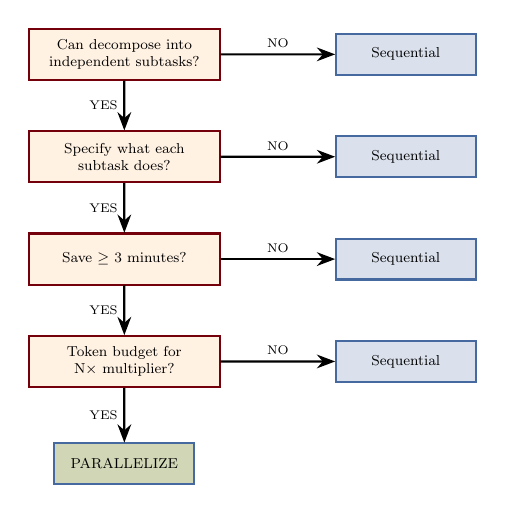
\begin{tikzpicture}[scale=0.65, transform shape,
            decision/.style={rectangle, draw=UofSCGarnet, thick, fill=UofSCSandstorm, text width=3.5cm, text centered, font=\footnotesize, minimum height=1cm},
            outcome/.style={rectangle, draw=UofSCAtlantic, thick, fill=UofSCAtlantic!20, text width=2.5cm, text centered, font=\footnotesize, minimum height=0.8cm}
        ]
            \node[decision] (d1) at (0,4) {Can decompose into independent subtasks?};
            \node[outcome] (seq1) at (5.5,4) {Sequential};

            \node[decision] (d2) at (0,2) {Specify what each subtask does?};
            \node[outcome] (seq2) at (5.5,2) {Sequential};

            \node[decision] (d3) at (0,0) {Save $\geq$ 3 minutes?};
            \node[outcome] (seq3) at (5.5,0) {Sequential};

            \node[decision] (d4) at (0,-2) {Token budget for N$\times$ multiplier?};
            \node[outcome] (seq4) at (5.5,-2) {Sequential};

            \node[outcome,fill=UofSCHorseshoe!30] (par) at (0,-4) {PARALLELIZE};

            \draw[myarrow] (d1) -- node[above,font=\scriptsize]{NO} (seq1);
            \draw[myarrow] (d1) -- node[left,font=\scriptsize]{YES} (d2);
            \draw[myarrow] (d2) -- node[above,font=\scriptsize]{NO} (seq2);
            \draw[myarrow] (d2) -- node[left,font=\scriptsize]{YES} (d3);
            \draw[myarrow] (d3) -- node[above,font=\scriptsize]{NO} (seq3);
            \draw[myarrow] (d3) -- node[left,font=\scriptsize]{YES} (d4);
            \draw[myarrow] (d4) -- node[above,font=\scriptsize]{NO} (seq4);
            \draw[myarrow] (d4) -- node[left,font=\scriptsize]{YES} (par);
        \end{tikzpicture}
    \end{center}
\end{frame}

% ----------------------------------------------------------------------------
\begin{frame}{Next Steps and Further Learning}
    \begin{columns}[T]
        \begin{column}{0.48\textwidth}
            \textbf{Immediate Next Steps}
            \begin{enumerate}
                \footnotesize
                \item Identify a parallelizable task
                \item Use templates from this presentation
                \item Measure results (time, tokens, quality)
                \item Document what you learned
            \end{enumerate}

            \vspace{0.3cm}
            \textbf{Short-Term Goals (2--3 weeks)}
            \begin{itemize}
                \footnotesize
                \item Master 3-agent research pattern
                \item Master 3-agent code review pattern
                \item Use in at least 5 distinct tasks
                \item Build personal template library
            \end{itemize}
        \end{column}
        \begin{column}{0.48\textwidth}
            \textbf{Development Path}

            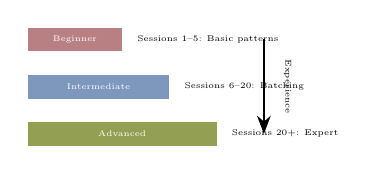
\begin{tikzpicture}[scale=0.6, transform shape]
                % Beginner
                \fill[UofSCGarnet!50] (0,3) rectangle (2,3.5);
                \node[font=\tiny,white] at (1,3.25) {Beginner};
                \node[font=\tiny,right] at (2.2,3.25) {Sessions 1--5: Basic patterns};

                % Intermediate
                \fill[UofSCAtlantic!70] (0,2) rectangle (3,2.5);
                \node[font=\tiny,white] at (1.5,2.25) {Intermediate};
                \node[font=\tiny,right] at (3.2,2.25) {Sessions 6--20: Batching};

                % Advanced
                \fill[UofSCHorseshoe!70] (0,1) rectangle (4,1.5);
                \node[font=\tiny,white] at (2,1.25) {Advanced};
                \node[font=\tiny,right] at (4.2,1.25) {Sessions 20+: Expert};

                % Arrow
                \draw[myarrow,thick] (5,3.25) -- (5,1.25);
                \node[font=\tiny,rotate=-90] at (5.5,2.25) {Experience};
            \end{tikzpicture}

            \vspace{0.3cm}
            \textbf{Questions to Explore}
            \begin{itemize}
                \footnotesize
                \item What tasks parallelize best in your domain?
                \item Optimal team size for your work?
                \item How to measure quality improvements?
            \end{itemize}
        \end{column}
    \end{columns}
\end{frame}

% ============================================================================
% APPENDIX
% ============================================================================
\appendix

% ----------------------------------------------------------------------------
\begin{frame}[fragile]{Appendix A: Quick Reference Templates}
    \begin{columns}[T]
        \begin{column}{0.48\textwidth}
\begin{lstlisting}[style=prompt,title={\footnotesize Three-Agent Research}]
Run 3 agents in parallel:
Agent 1 - Codebase Explorer:
  Explore [PROJECT] for [TOPIC].
Agent 2 - Literature Researcher:
  Search papers/docs for [TOPIC].
Agent 3 - Pattern Identifier:
  Find similar implementations.
After completion, synthesize.
\end{lstlisting}
        \end{column}
        \begin{column}{0.48\textwidth}
\begin{lstlisting}[style=prompt,title={\footnotesize Code Review Panel}]
Review from 3 angles:
Agent 1 - Correctness:
  Check logic, edge cases, errors.
Agent 2 - Style:
  Check readability, naming.
Agent 3 - Performance:
  Check efficiency, algorithms.
Consensus: Issues 2+ agree on?
\end{lstlisting}
\end{column}
    \end{columns}
\end{frame}

% ----------------------------------------------------------------------------
\begin{frame}{Appendix B: Troubleshooting Guide}
    \footnotesize
    \begin{tabular}{p{3.5cm}p{4cm}p{4cm}}
        \toprule
        \textbf{Problem} & \textbf{Cause} & \textbf{Fix} \\
        \midrule
        One agent times out & Unbalanced workload & Redistribute work evenly \\
        Contradictory results & Different interpretation & More specific instructions \\
        Synthesis fails & Format not specified & Specify exact output format \\
        Quality worse than seq & Vague instructions & Give focused roles \\
        Token cost too high & Too many agents & Reduce agent count \\
        Parallelization slower & Overhead exceeds savings & Use sequential for small tasks \\
        Empty agent output & Silent failure & Make requirements explicit \\
        \bottomrule
    \end{tabular}
\end{frame}

% ----------------------------------------------------------------------------
\begin{frame}{Appendix C: Metric Formulas}
    \begin{columns}[T]
        \begin{column}{0.48\textwidth}
            \textbf{Performance Metrics}
            \begin{align*}
                \text{Speedup} &= \frac{\text{Seq\_Time}}{\text{Par\_Time}} \\[0.5em]
                \text{Token\_Mult} &= \frac{\text{Par\_Tokens}}{\text{Seq\_Tokens}} \\[0.5em]
                \text{Cost/Min} &= \frac{\Delta\text{Tokens}}{\Delta\text{Time}}
            \end{align*}
        \end{column}
        \begin{column}{0.48\textwidth}
            \textbf{ROI Calculation}
            \begin{align*}
                \text{Time\_Value} &= \frac{\text{Min\_Saved}}{60} \times \text{Rate} \\[0.5em]
                \text{Token\_Cost} &= \frac{\text{Extra\_Tokens}}{10^6} \times \text{Cost} \\[0.5em]
                \text{ROI} &= \text{Time\_Value} - \text{Token\_Cost}
            \end{align*}

            \vspace{0.3cm}
            \textbf{Parallelization Worth If:}
            \begin{itemize}
                \footnotesize
                \item (Speedup $>$ 1.3) AND (Token\_Mult $<$ 3)
                \item OR Quality\_Improvement $>$ 20\%
            \end{itemize}
        \end{column}
    \end{columns}
\end{frame}

% ----------------------------------------------------------------------------
\begin{frame}
    \begin{center}
        \Huge\textcolor{UofSCGarnet}{Questions?}

        \vspace{1cm}

        \Large Part 7: Parallelization with Agents

        \vspace{0.5cm}

        \normalsize
        University of South Carolina\\
        Graduate Research Seminar
    \end{center}
\end{frame}

\end{document}
